\section{Particles - introduction and overview}
\subsection{What makes a particle}
\begin{figure}
\rotatebox{270}{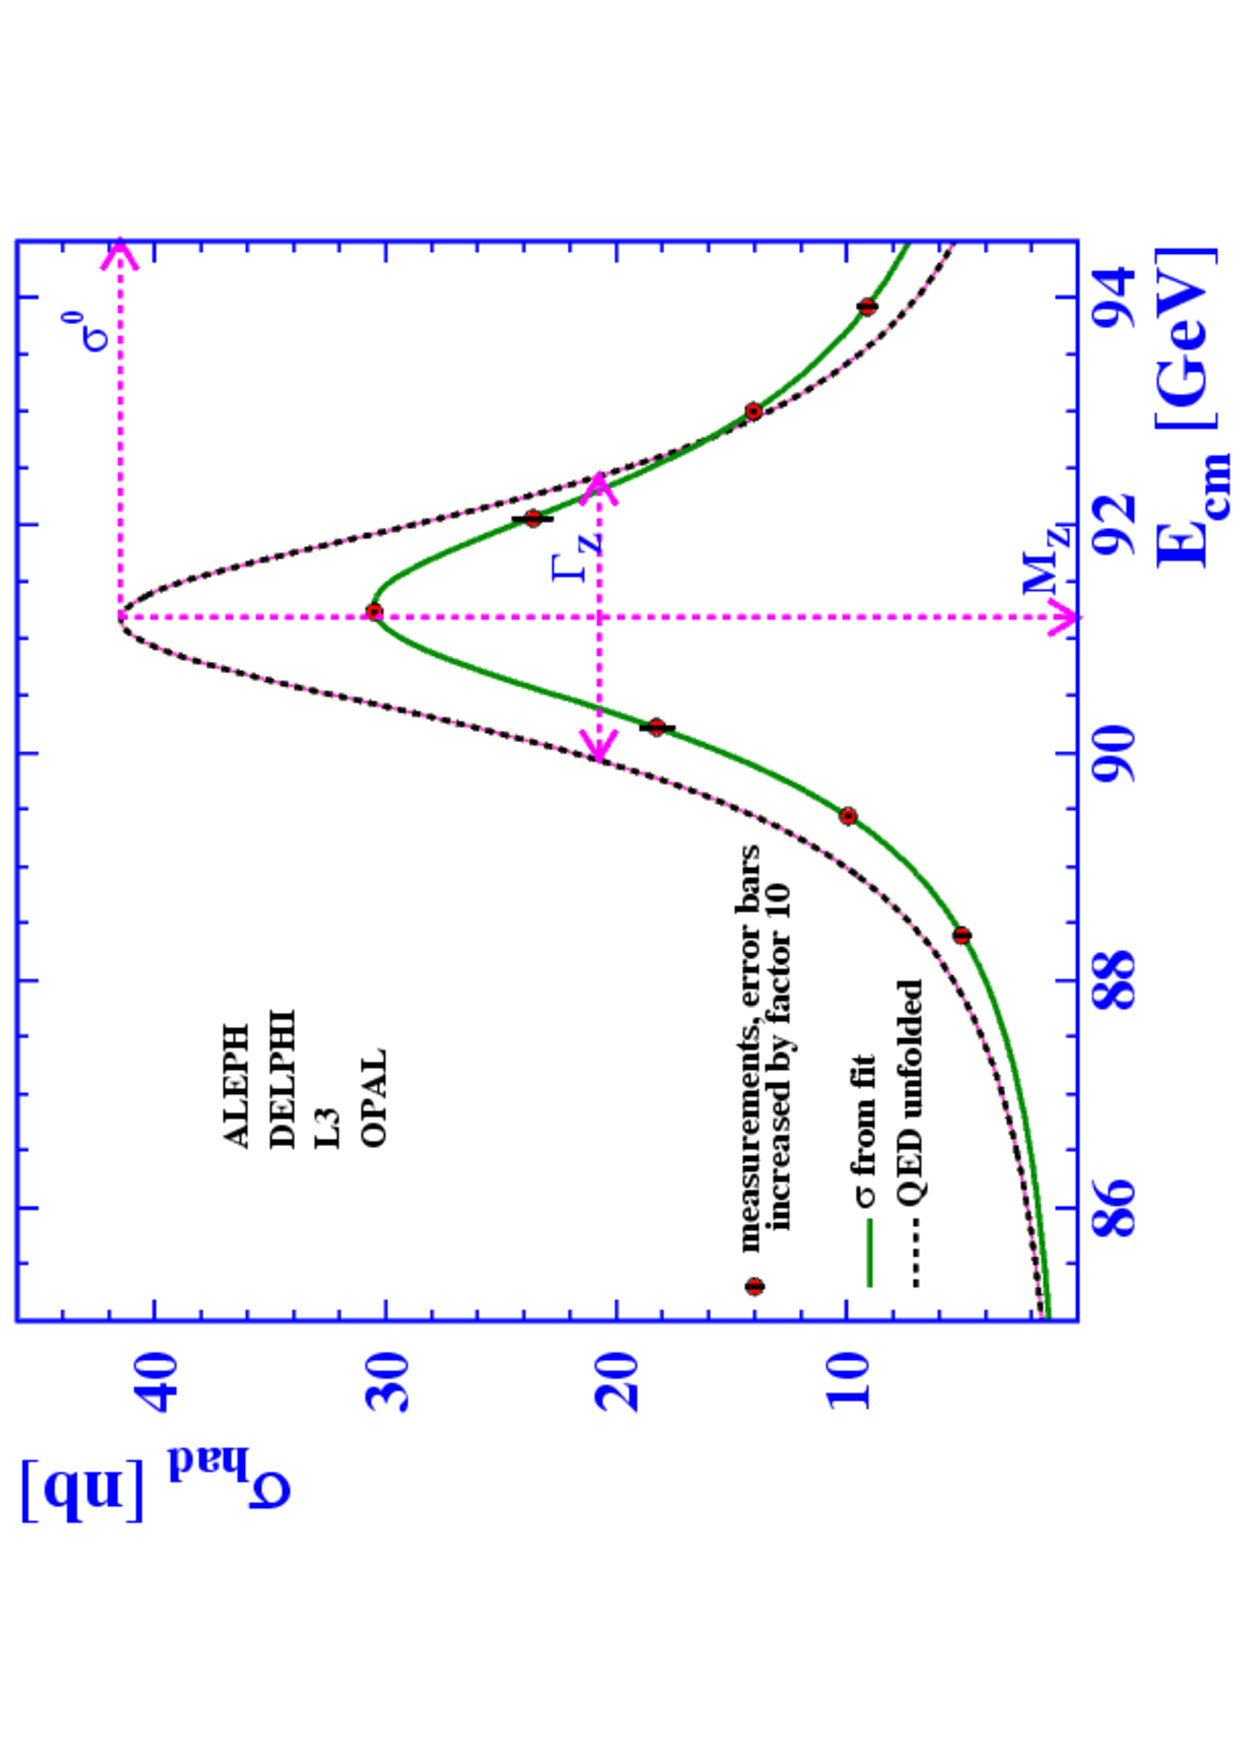
\includegraphics[width=0.6\textwidth]{fig/z_lineshape}}
\caption{The y-axis gives the cross section (proportional to probability) to produce a $Z$ particle at LEP at a given mass. To first order: ignore the green solid line, only look at the red/black broken line. (The solid green line is the uncorrected measurement of $Z$ production versus centre of mass energy of the $e^+ e^-$ beam, the red-black dotted line is $Z$ production as a function of true energy used to make the $Z$, which is subtly different because sometimes electrons and positrons radiate off photons before they collide, so that the energy available to make a $Z$ is a bit less than the beam energy.) The crucial point is that for unstable particles, we need to know both, the mean mass and the width.\label{fig:z_lineshape}}
\end{figure}
\begin{figure}
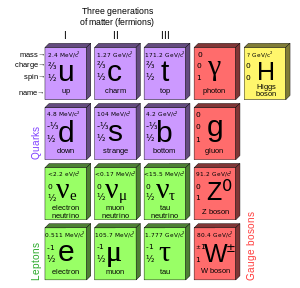
\includegraphics[width=0.6\textwidth]{fig/TheSM}
\caption{The particles of the Standard Model, and some of their basic properties, such as mass and electric charge. All electrically charged particles couple to the photon and thus interact electromagnetically. While the electric charge is given, the colour charge and weak charge are omitted in this figure. All quarks and gluons carry colour charge and thus couple to gluons (that's right, the gluons couple also to themselves), and thus interact strongly. The other particles do not. All fermions, as well as Z and W carry a weak charge, which means they couple to W and Z and can interact weakly.\label{fig:SM}}
\end{figure}


What are particles? And in particular, what are fundamental particles? We view fundamental particles a point-like objects without any internal structure. Surely, such simple objects cannot have many properties. And indeed, they are characterised fully by just a few parameters. Let us first look the 'intrinsic' properties, that are the same in any reference frame. A key property of a particle is its mass. However, for unstable particles, we need to be a bit careful, as, due to Heisenberg's uncertainty principle $\Delta E\Delta t \ge \half \hbar$, their mass (energy) is not fixed if $\Delta t \neq \infty$. The consequence of this is illustrated in Fig~\ref{fig:z_lineshape}, showing how $Z$ bosons are produced with different masses. The probability that a $Z$ will have a certain mass is described by a lineshape with two parameters: The mean mass $M$, and the width, $\Gamma$. $\Gamma$ is related to the mean lifetime of the particle, $\tau$, by 
\begin{equation}
    \tau = \frac{\hbar}{\Gamma}.
\end{equation}

Another important property of a particle is its spin. Particles with half-integer spin quantum number ($\frac{1}{2}, \frac{3}{2}, \ldots$)  are fermions, those with full-integer spin quantum number (0, 1, 2...) are bosons, which fundamentally changes their properties. Also, the spins of a particle and its decay products affect the angular distribution of the particle's decay products. 

There are further quantum numbers which can only have discrete values.They are all related to symmetries, such has how the particle behaves under parity (effectively mirror reflection), or what their wavefunction does when we swap particles with antiparticles.  We will discuss these later. Finally, the interactions of a particle with other particles are determined by its charges under the strong, the weak and the electromagnetic interaction.

And then there properties that depend on the reference frame and describe the motion of a particle. They are its four momentum (actually, if we know the mass, the 3-momentum is enough, but as mentioned above, for unstable particles the mass can vary case-by-case), and the projection of the spin onto some axis. In particle physics, we  take the projection of the spin onto the the axis defined by the particle's momentum. This quantity (multiplied by two) is called helicity. The (fairly deep) reason for this choice over the more familiar projection onto the $z$ axis will be discussed in the context of the Dirac equation.

%%Composite particles have additional properties, such as size, shape, etc. In some cases, composite particles can look like fundamental particles. This is the case when the energies involved in the interaction are such that the associated wavelengths are much larger than the size of the composite particle. This is why in atomic physics (energies of a few 10s of $eV$, the nucleus looks like a point particle to a good approximation. In nuclear physics (energies of $MeV$), nuclei are complex objects, but protons and neutrons are usually treated as structureless particles. And at the LHC (energies of several $TeV$), the proton looks like a highly complicated object formed of gluons and quarks.

Figure \ref{fig:SM} lists the fundamental particles we know about, with some of their properties. From these particle properties, we can calculate how the particles interact with each other. The tool we use for this are Feynman diagrams.

\subsection{Feynman diagrams and Feynman rules}

Feynman diagrams are a graphical representation of what is in fact a series expansion (like a Taylor expansion) of the full theory. The number of vertices in the diagram represents the order of the term in that expansion that the Feynman diagram represents. Most of the time we'll only deal with the lowest order term.

Each Feynman diagram has an exact mathematical value, which corresponds to a quantum mechanical transition amplitude, which is in general a complex number. If several Feynman diagrams contribute to the same process, their complex values need to be added up to get the full amplitude $\mathcal{M}_{fi} = A_1 + A_2 + \ldots$. A transition rate proportional to the magnitude of this number, squared:
\begin{equation}
    R \propto \left| \mathcal{M}_{fi} \right|^2
\end{equation}
The $\mathcal{M}_{fi}$ stands here for "matrix element", which is the total complex amplitude for a transition from one initial state $i$ to a final state $f$.

Evaluating Feynman diagrams can be quite a messy operation. We will here adopt the following PGA (pretty good approximation): \textbf{we will estimate Feynman diagrams \emph{ignoring spin}.} This simplifies things immensely (no gamma matrices). Our results will be good approximations as long as spin does not matter. We won't be very good at getting angular distributions right with this, but for total rates we will get good estimates in most cases. There is one significant exception in the weak interaction (helicity suppression), but we will deal with that separately. Several things will even be exactly right, such as the weak-interaction phases introduced in the context of charge-symmetry violation (see later).

\subsection{Drawing and Evaluating Feynman Diagrams}

\paragraph{Time runs from left to right in the sense that:}
\begin{itemize}
\item LHS of the diagram is the initial state
\item RHS of the diagram is the final state
\item Middle of the diagram is how it happened
\end{itemize}

\paragraph{Anti-particle arrows should point in negative time direction} for example for the $e^+e^-\to \mu^+\mu^-$ process we have
\begin{center}
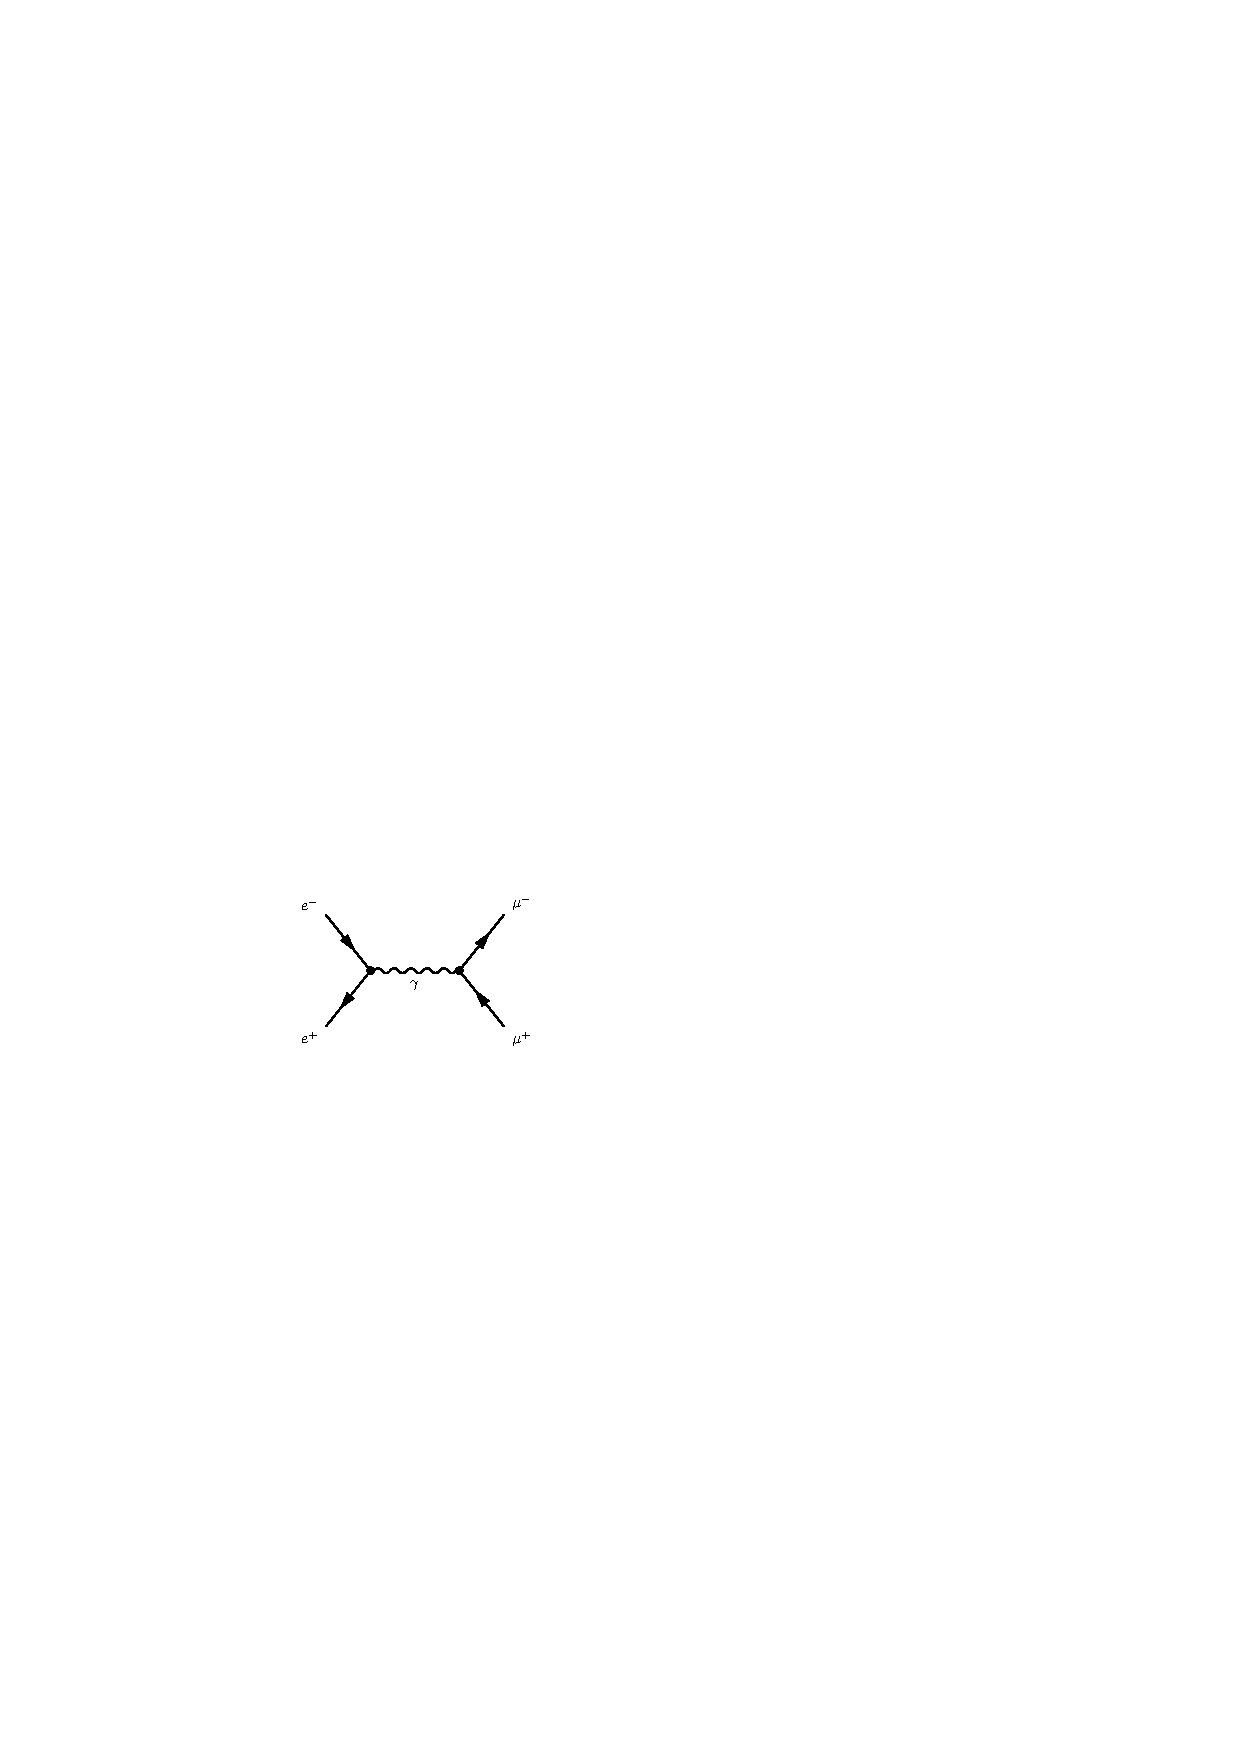
\includegraphics[width=0.5\textwidth]{fig/forcerange/eetomm.pdf}
\end{center}

\paragraph{At each vertex, 4-momenta are conserved}

\paragraph{Each vertex contributes a coupling strength factor $g$ which is proportional to the charge of the particle in question.}
In EM interactions $g$ is simply the electric charge; for an electron it's $e=\sqrt{4\pi\alpha_{EM}}$, for an upquark it's $e= - \frac{2}{3}\sqrt{4\pi\alpha_{EM}}$, for a down quark it's $e= + \frac{1}{3}\sqrt{4\pi\alpha_{EM}}$. Here $\alpha_{EM}$ is the fine structure constant $\alpha_{\rm EM}=\frac{1}{137}$. So for the example above, the process occurs at a rate proportional to $\alpha_{\rm EM}^2$.

\paragraph{Each intermediate particle (connecting 2 vertices) contributes a factor $\frac{1}{q^2 - m^2}$} where $q$ is the particle's four-momentum. The intermediate particles is virtual, and usually $E^2 \neq p^2+m^{2}$. The intermediate particle is said to be ``off-shell''. 

Below a graphical summary of our simplified (no spin) Feynman rules for QED:\\
\begin{tabular}{cc}
\textbf{Vertices} & \textbf{propagators} \\
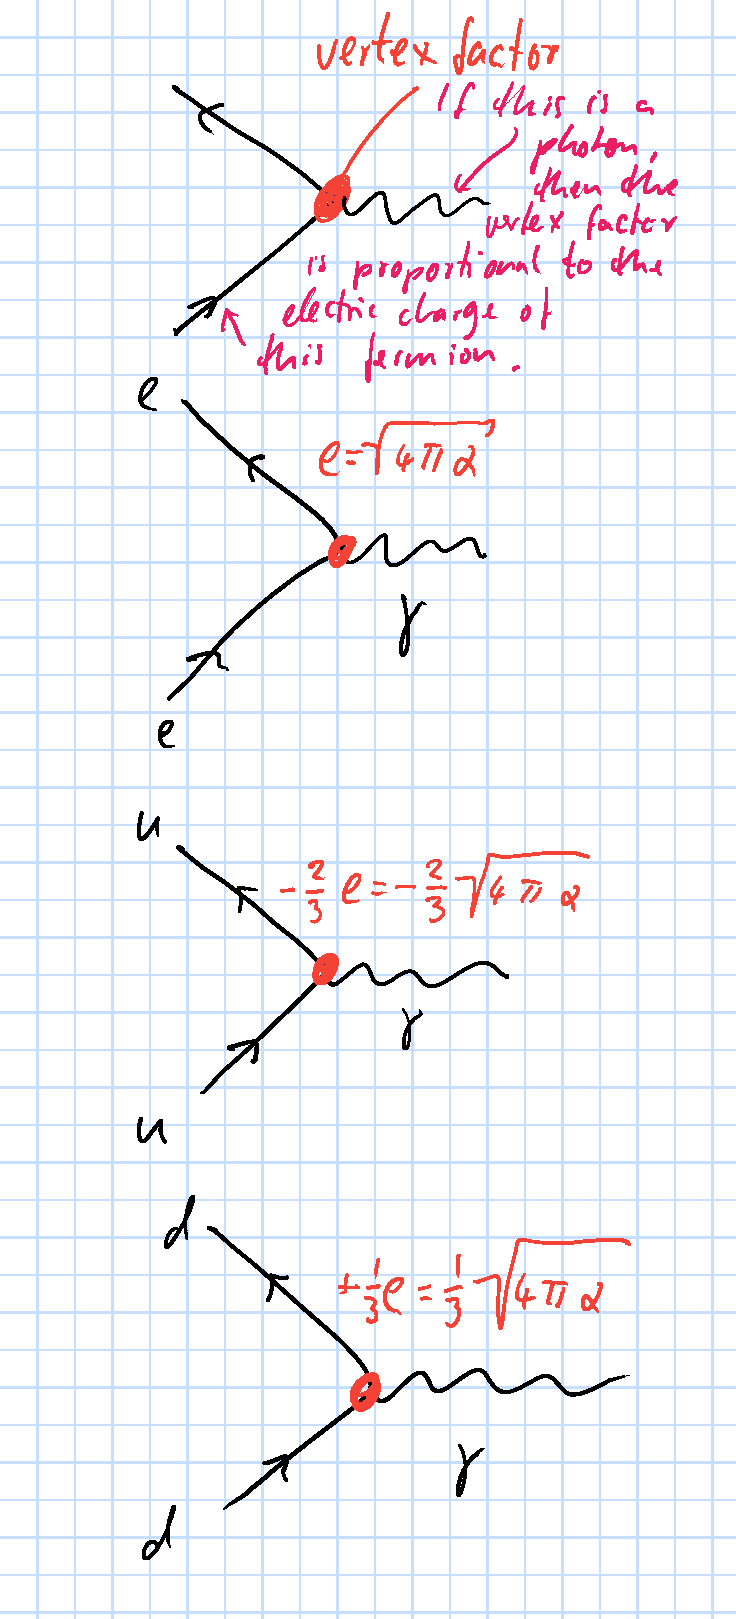
\includegraphics[width=0.4\textwidth]{fig/VertexFactorsQED}
&
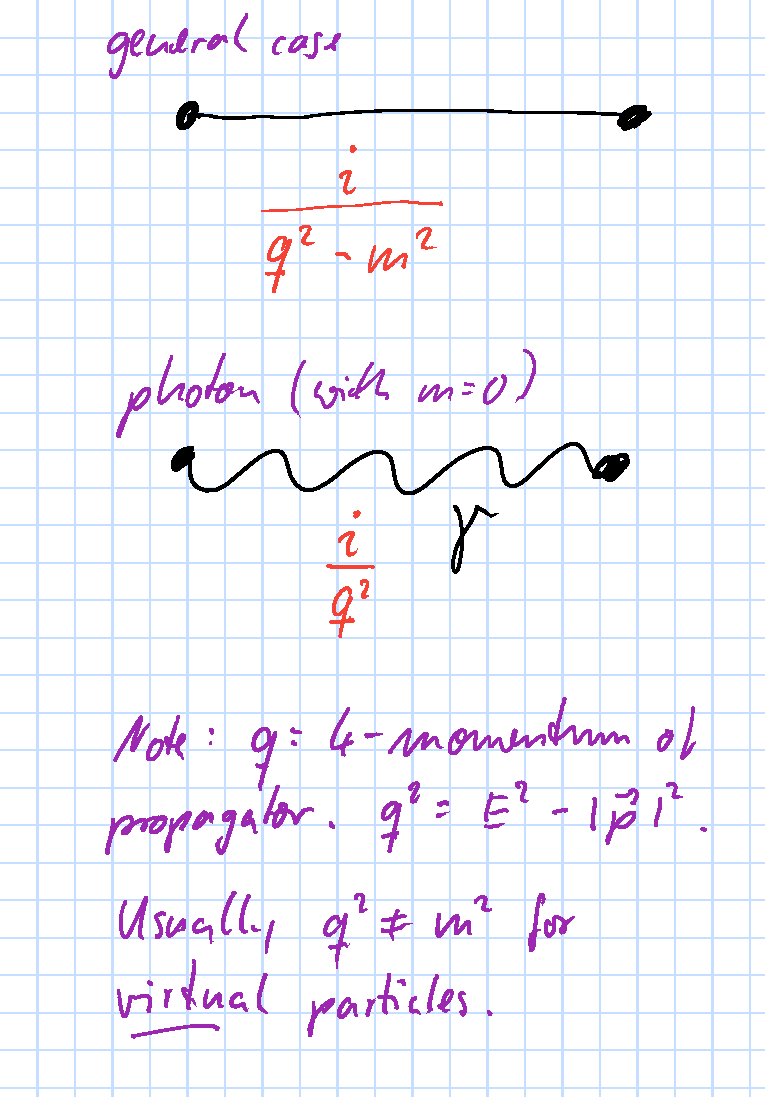
\includegraphics[width=0.58\textwidth]{fig/FeynmanPropagators}
\end{tabular}
Note that time goes from left to right and we represent antiparticles as particles going backwards in time. So an $e^-$ ($u$) is an electron (up quark) going from left two right, while an $e^+$ ($\overline{u}$) is an electron (up quark) going from right to left. You \emph{can} add labels like $\overline{u}$ next to lines going from right to left to emphasise it's an anti-particle, but you do not need to (and I usually won't), the direction of the arrow makes it all clear.

These can be stuck together to form all sorts of processes, for example $e^+ e^- \to u \overline{u}$ scattering:
\\
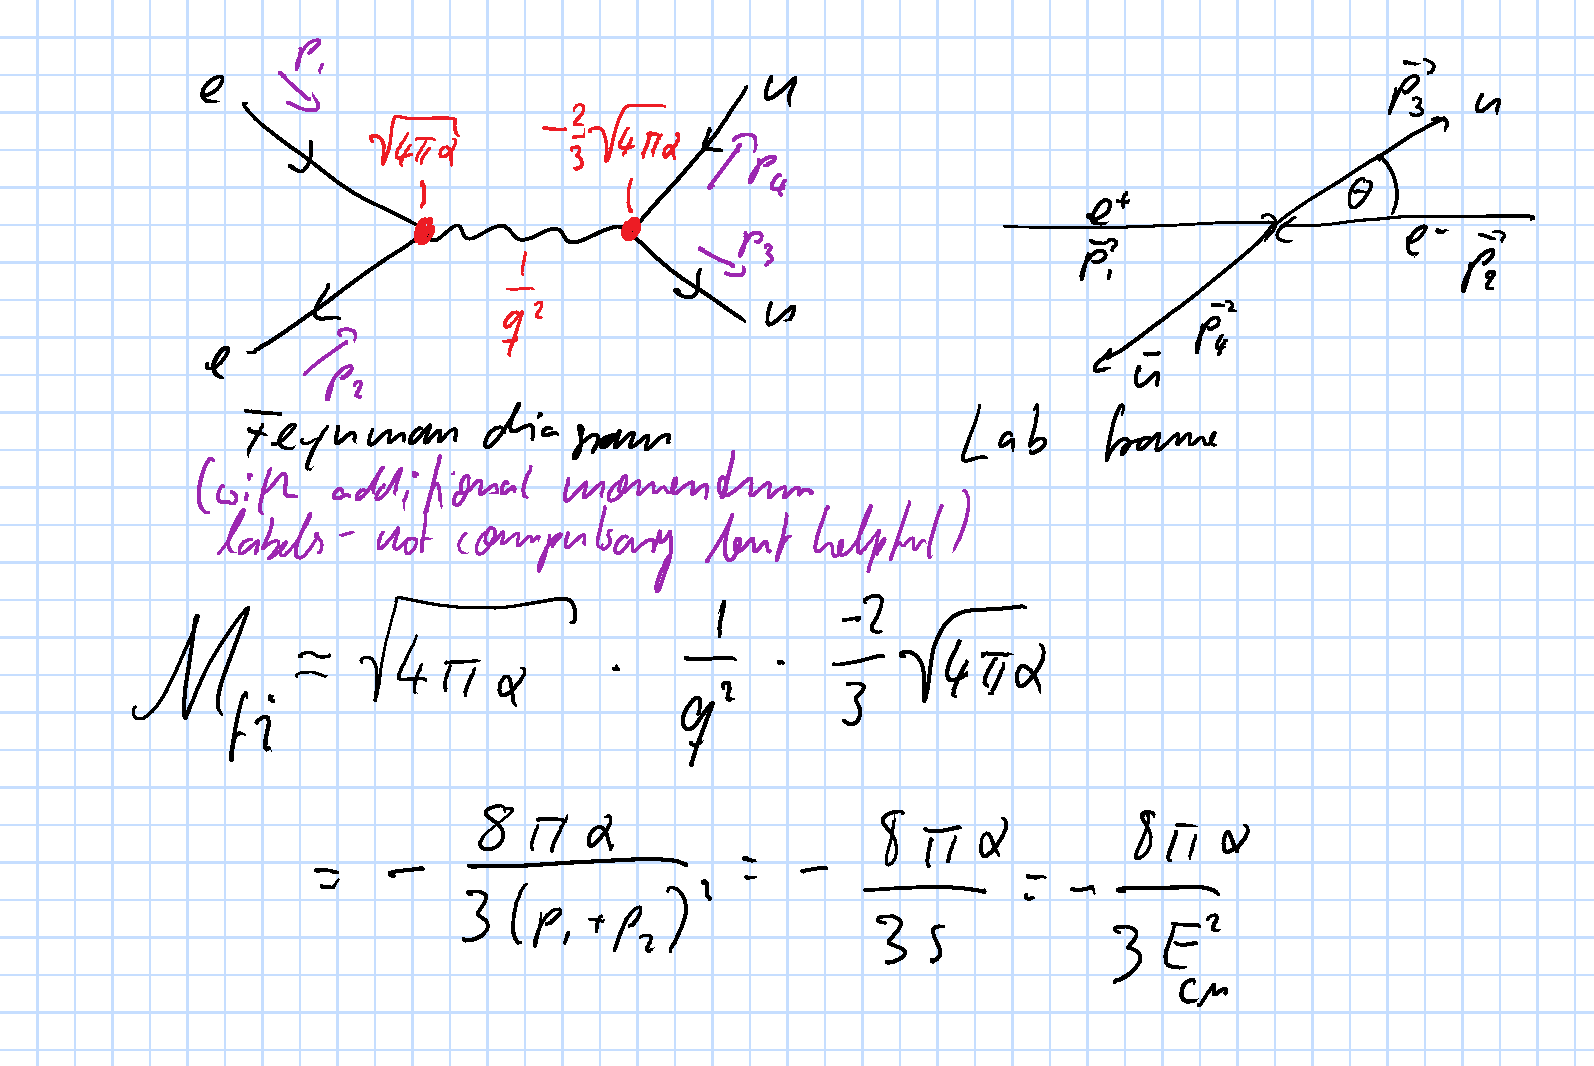
\includegraphics[width=0.9\textwidth]{fig/ExampleQED_1}

\exercise{
Draw and evaluate the Feynman diagrams in terms of the cm energy $E_{cm}=\sqrt{s}$ for these processes:
\begin{enumerate}
\item $e^+ e^- \to \mu^+ \mu^-$
\item $e^- \mu- \to e^- \mu^-$
\end{enumerate}
\inlineAnswer{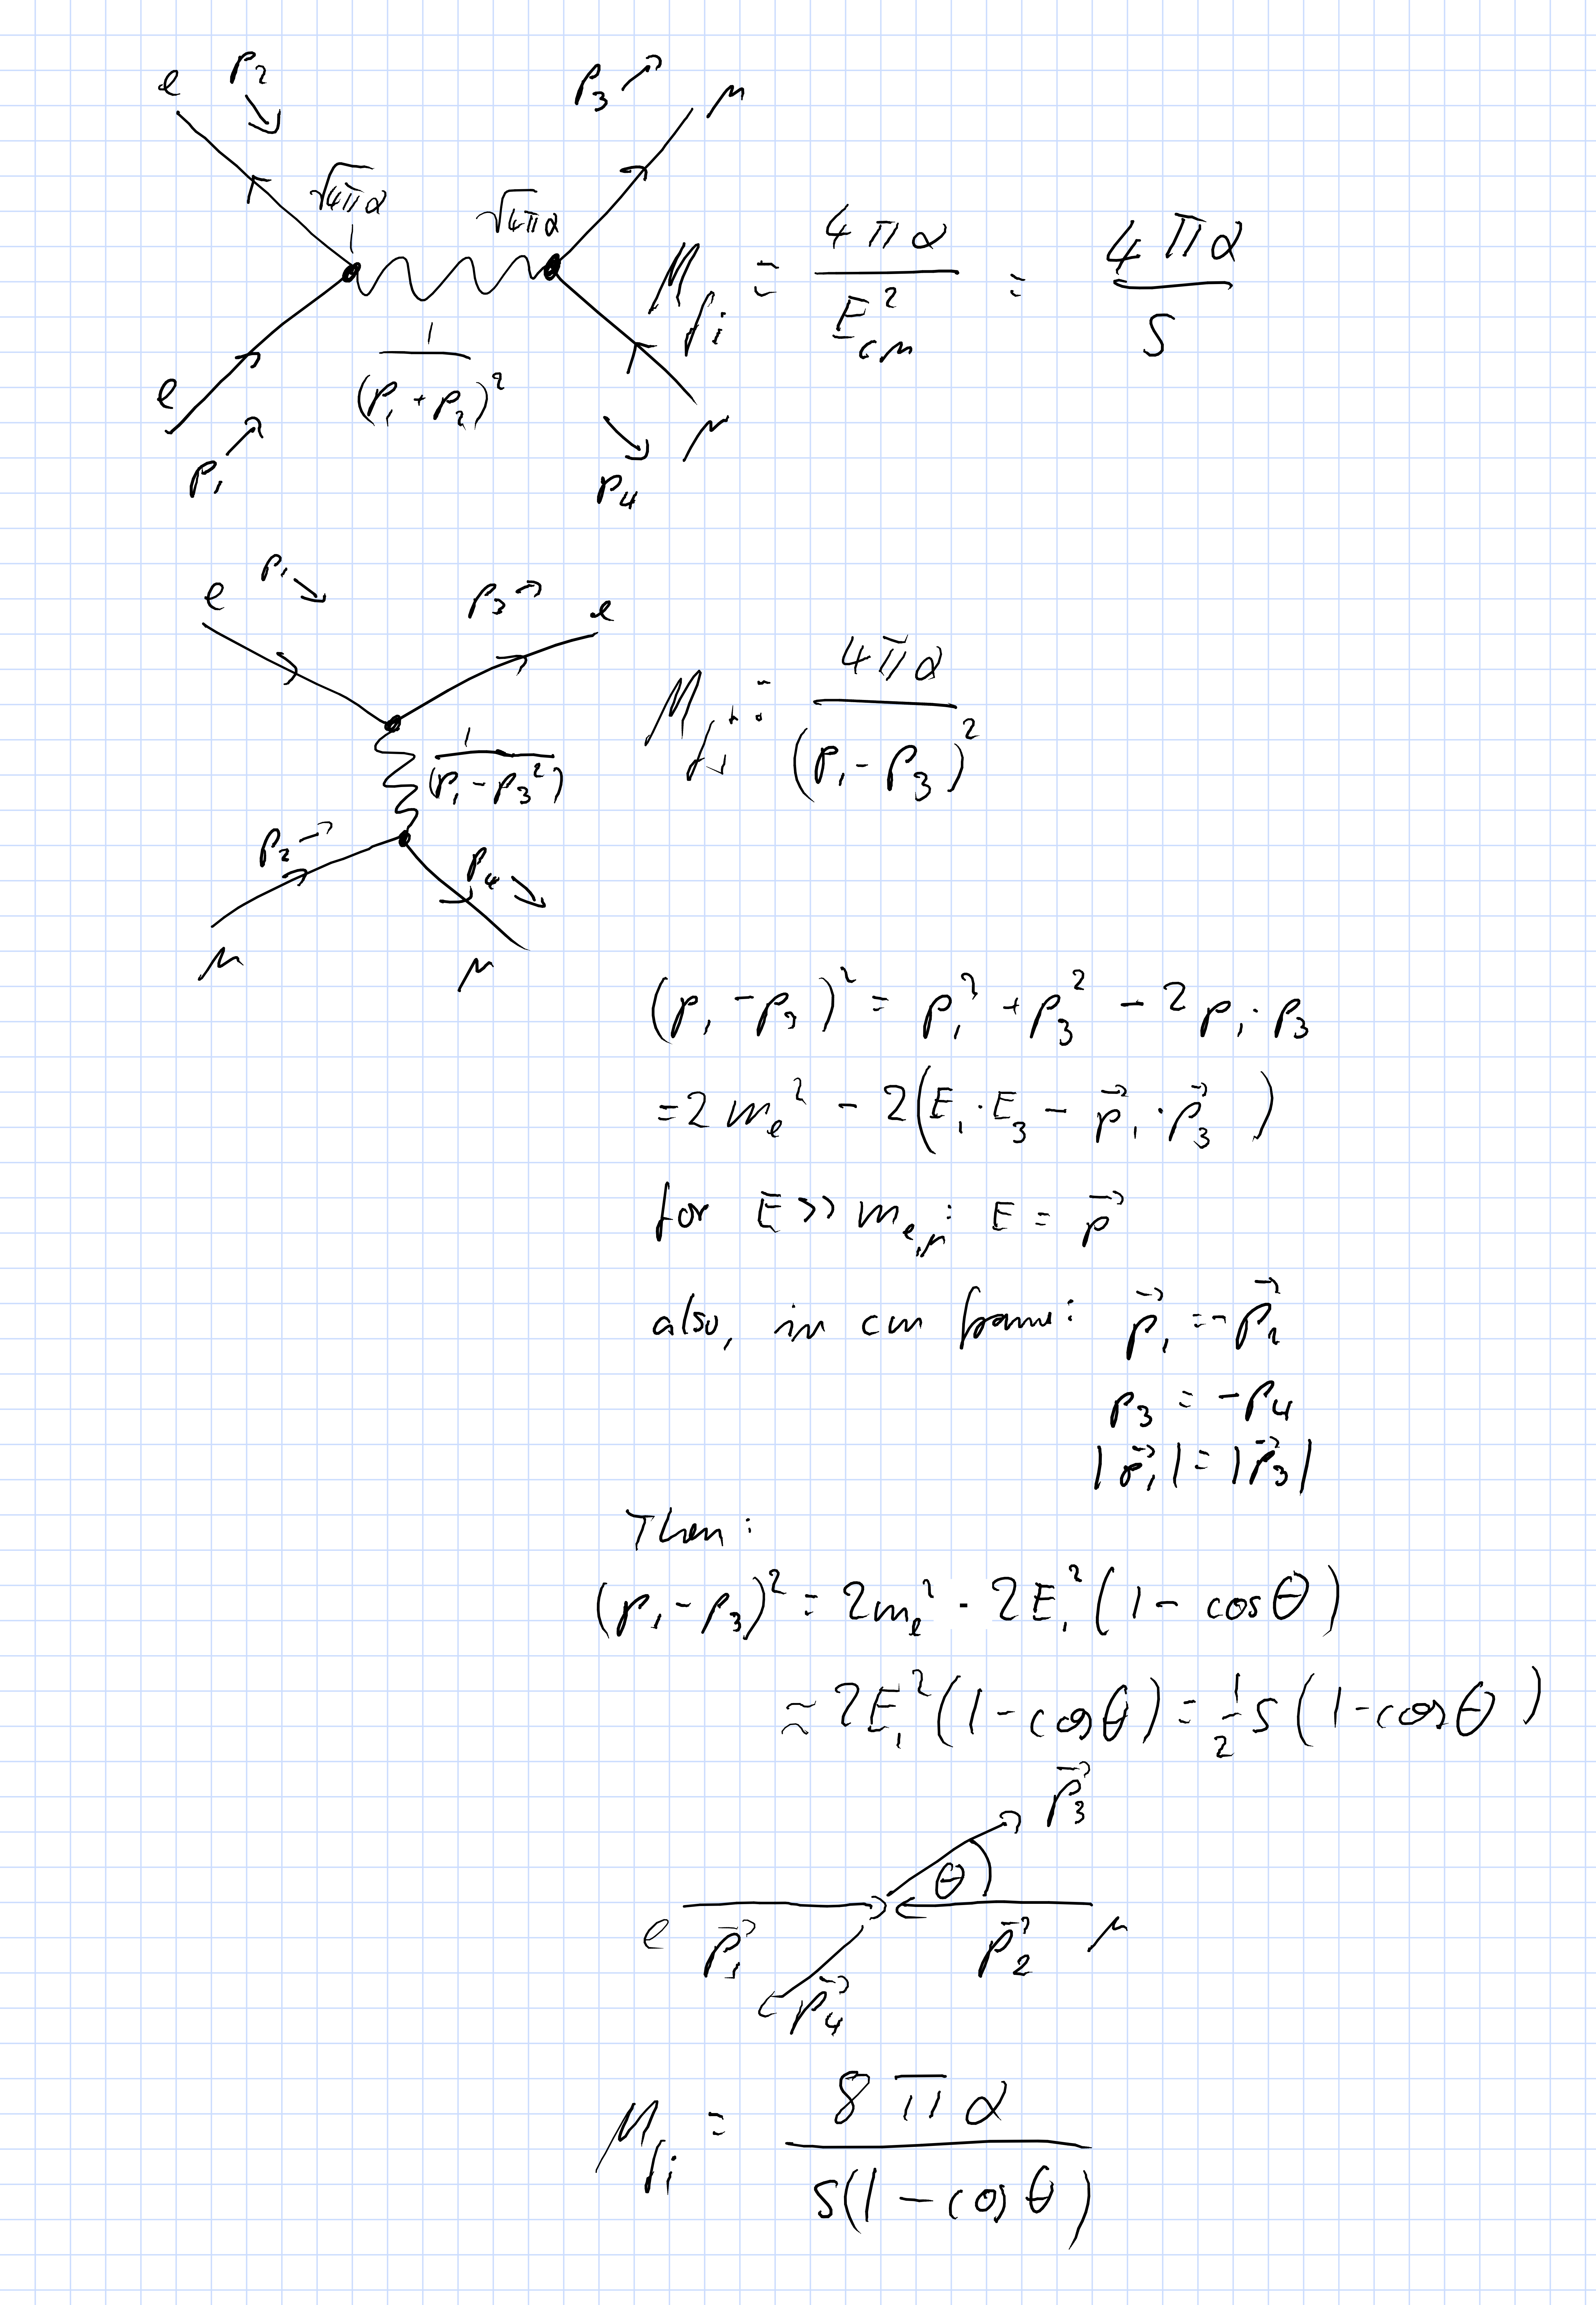
\includegraphics[width=0.8\textwidth]{fig/FeynmanFirstRevisionExercises.png}}
}

A nice introduction to drawing Feynman diagrams (and other topics in particle physics) can be found here: \href{http://www.quantumdiaries.org/2010/02/14/lets-draw-feynman-diagams}{http://www.quantumdiaries.org/2010/02/14/lets-draw-feynman-diagams}.
